\documentclass{sig-alternate}
\usepackage{amsmath,amssymb}
\usepackage{graphicx}
\usepackage{hyperref}
\usepackage{color}

\newcommand{\comment}[1]{}
\newcommand{\compiler}{DBCC}
\newcommand{\todo}[1]{\textcolor{red}{#1}}
\newcommand{\feature}[1]{\textbf{#1.}}
\newcommand{\tuple}[1]{{\langle#1\rangle}}
\newcommand{\bigsum}{bigsum}

\newtheorem{theorem}{Theorem}[section]
\newtheorem{metatheorem}{Metatheorem}[section]
\newtheorem{example}[theorem]{Example}
%\newtheorem{algorithm}[theorem]{Algorithm}
\newtheorem{definition}[theorem]{Definition}
\newtheorem{proposition}[theorem]{Proposition}
\newtheorem{property}[theorem]{Property}
\newtheorem{corollary}[theorem]{Corollary}
\newtheorem{lemma}[theorem]{Lemma}
\newtheorem{remark}[theorem]{Remark}
\newtheorem{conjecture}[theorem]{Conjecture}
\newtheorem{proviso}[theorem]{Proviso}

\begin{document}
\title{DBCC: Compiling Databases for High-Performance View Maintenance and Update Stream Processing}
\numberofauthors{2}
\author{
\alignauthor Yanif Ahmad\\
    \affaddr{Computer Science Dept.}\\
    \affaddr{Cornell University}\\
    \email{yanif@cs.cornell.edu}
\alignauthor Christoph Koch\\
    \affaddr{Computer Science Dept.}\\
    \affaddr{Cornell University}\\
    \email{koch@cs.cornell.edu}
}
\maketitle



In recent years, algorithmic trading systems have come to account for a majority
of volume traded at the major US and European financial markets (for instance,
for 73\% of all US equity trading volume in the first quarter of 2009
\cite{Iati2009}). The success of automated trading systems depends critically on
strategy processing speeds: trading systems that react faster to market events
tend to make money at the cost of slower systems. Unsurprisingly, algorithmic
trading has become a substantial source of business for the IT industry; for
instance, it is the leading vertical among the customer bases for high-speed
switch manufacturers (e.g., Arista \cite{Becht2010}) and data stream processing.




A typical algorithmic trading system is run by mathematicians who develop
trading strategies and by programmers and systems experts who implement these
strategies to perform fast enough, using mainly low-level programming languages
such as C. Developing trading strategies requires a feedback loop of simulation,
back-testing with historical data, and strategy refinement based on the insights
gained. This loop, and the considerable amount of low-level programming that it
causes, is the root of a very costly {\em productivity bottleneck}\/: in fact,
the number of programmers often exceeds the number of strategy designers by
an order of magnitude.


Trading algorithms often perform a considerable amount of data crunching
and statistical processing that could in principle be implemented using SQL
views, coupled with some relatively straightforward control and trading logic.
%
Differently from other areas of finance such as technical analysis,
where stream processing engines
\cite{abadi-vldbj:03,motwani-cidr:03} can be applied,
data processing in trading algorithms using views cannot be performed by DBMS or
data stream processing systems today: the former are not able to (1) {\em update
their views at the required rates}\/ (for popular stocks, hundreds of orders per
second may be executed, even outside burst times) and the latter are not able to
(2) {\em maintain large enough data state}\/ and support suitable query
languages (non-windowed SQL aggregates) on this state.

%
A data management system that could handle these two requirements would yield a
very substantial productivity increase that can be directly monetized -- the
holy grail of algorithmic trading.

Trading algorithms often perform a considerable amount of data crunching that
could in principle be implemented as SQL views, but cannot be achieved by DBMS
or data stream processing systems today: DBMS are not able to (1) {\em update
their views at the required rates}\/ (for popular stocks, hundreds of orders per
second may be executed, even outside burst times) and stream engines are not
able to (2) {\em maintain large enough data state}\/ and support suitable query
languages (non-windowed SQL aggregates) on this state.
A data management system fulfilling these two requirements would yield a very
substantial productivity increase that can be directly monetized -- the holy
grail of algorithmic trading.



To understand the need to maintain and query a large data state, note that
many stock exchanges provide a detailed view of the market microstructure
through complete bid and ask {\em limit order books}. The bid order book is a
table of purchase offers with their prices and volumes, and correspondingly the
ask order book indicates investors' selling orders. Exchanges execute trades by
matching bids and asks by price and favoring earlier timestamps. Investors
continually add, modify or withdraw limit orders, thus one may view order books
as relational tables subject to high update volumes. The availability of order
book data has provided substantial opportunities for automatic algorithmic
trading.





To illustrate this, we describe the Static Order Book Imbalance (SOBI) trading
strategy. SOBI computes a volume-weighted average price (VWAP) over those orders
whose volume makes up a fixed upper $k$-fraction of the total stock volume in
both bid and ask order books. SOBI then compares the two VWAPs and, based on
this, predicts a future price drift (for example a bid VWAP larger than an ask
VWAP indicates demand exceeds supply, and prices may rise). For simplicity, we
present the VWAP for the bids only:



\begin{verbatim}
select avg(b2.price * b2.volume) as bid_vwap
from   bids b2
where  k * (select sum(volume) from bids)
         > (select sum(volume) from bids b1
            where b1.price > b2.price);
\end{verbatim}
\comment{
Focusing on the $k$-fraction of the order book closest to the current price
makes the SOBI strategy less prone to attacks known as {\em axes}\/ (large
tactical orders far from the current price that will thus not be executed but
may confuse competing algorithms).
}


Coming back to our two desiderata, for trading algorithms to be successful, (1)
views such as VWAP need to be maintained and monitored by the algorithms at or
close to the trading rate. However, (2) the views cannot be expressed through
time-, row- or punctuation-based window semantics.





\section{Query Compilation}

\def\algsum{\mathrm{sum}}
\def\algagg{\mathrm{agg}}
\def\algtop{\mathrm{top}}
\def\algtopk{\mathrm{topk}}

\def\algsumr{\mbox{sumr}}
\def\algsumf{\mbox{sumf}}
\def\distinct{\mbox{distinct}}
\def\routerjoin{\bowtie\!=}

We now present \compiler's compilation algorithm through an example
illustrating how queries are turned into efficient procedural code. Our
compilation framework applies to the core relational algebra and group-by
aggregates, and uses a custom query algebra to define map data structures. These
maps are closely related to views definable by SQL aggregate group-by queries but
at the same time are main memory data structures that are easy to access in
applications. Due to space limitations we only present the small fraction
of our map algebra transformations used to derive code for our example query.

\noindent\textbf{Compilation example.} Consider the query below on three
relations and schemas $R(A,B), S(B,C), T(C,D)$:

\begin{verbatim}
select sum(A*D) from R, S, T
where R.B=S.B and S.C=T.C
\end{verbatim}

Next, given the data and query model above, relations $R, S, T$ are
manipulated via update streams which consist of the standard requests
of inserting, updating and deleting tuples. For ease of presentation, we can
consider updates as pairs of delete and insert requests. We start with handling
an insert to the relation $R$, with a tuple $\{\tuple{a,b}\}$. Assuming
the variable $q$ maintains the query result, we can show:

\smallskip
Insert R(a,b):
\begin{eqnarray*}
\Delta q &=& \algsum_{A*D}(\{\tuple{a,b}\} \bowtie S \bowtie T)
\\ &=&
\algsum_{A*D}(\{a\} \times \sigma_{B=b}(S) \bowtie T)
\\ &=&
\algsum_{a*D}(\sigma_{B=b}(S) \bowtie T)
\\ &=&
a * \underbrace{\algsum_{D}(\sigma_{B=b}(S) \bowtie T)}_{q_D[b]}
\end{eqnarray*}

Above $q_D[b]$ is an example of a map that we use to compute the change in query
result $q$, a map with key-value pair entries of keys $b$, and values defined as
the result of the query: $\algsum_{D}(\sigma_{B=b}(S) \bowtie T)$. While we do
not go into the full details of the derivation validity, we can see it is a
simplification of the original query by considering the relation $R$ as a
singleton relation $\{\tuple{a,b}\}$. We can symmetrically derive for inserting
into relation $T$ as: $\Delta q = d * q_A[c]$, resulting in a map
$q_A[c] = \algsum_{A}(R \bowtie \sigma_{C=c}(S))$. The insertion to $S$ is:

\smallskip
Insert S(b,c):
\begin{eqnarray*}
\Delta s &=& \algsum_{A*D}(R \bowtie \{\tuple{b,c}\} \bowtie T)
\\ &=&
\algsum_{A*D}(\sigma_{B=b}(R) \times \sigma_{C=c}(T))
\\ &=&
\underbrace{\algsum_{A}(\sigma_{B=b}(R))}_{q_A[b]} *
\underbrace{\algsum_{D}(\sigma_{C=c}(T))}_{q_D[c]}
\end{eqnarray*}



\begin{figure*}[tb]
\begin{center}
\begin{tabular}{|l|l|l|l|l|l|}
\hline
Recursion level & Event & Query $q$ & Code for $\Delta q$ & Maps & Map
definition\\
\hline
1 & $+R$ & $\algsum_{A*D}(R \bowtie S \bowtie T)$
& $a*q_D[b]$ & $q_D[b]$ & $\algsum_{D}(\sigma_{B=b}(S) \bowtie T)$
\\
\hline
1 & $+S$ & $\algsum_{A*D}(R \bowtie S \bowtie T)$
& $q_A[b] * q_D[c]$ & $q_A[b]$ & $\algsum_{A}(\sigma_{B=b}(R))$
\\
& & & & $q_D[c]$ & $\algsum_{D}(\sigma_{C=c}(T))$
\\
\hline
1 & $+T$ & $\algsum_{A*D}(R \bowtie S \bowtie T)$
& $d*q_A[c]$ & $q_A[c]$ & $\algsum_{A}(R \bowtie \sigma_{C=c}(S))$
\\
\hline
2 & $+R$ & $\algsum_{A}(R \bowtie \sigma_{C=c}(S))$
& $\mbox{foreach($c$): } a * q_1[b,c]$ & $q_1[b,c]$ &
$\algsum_{1}(\sigma_{BC=bc}(S))$
\\
2 & $+R$ & $\algsum_{A}(\sigma_{B=b}(R))$
& $a$ & & \\
\hline
2 & $+S$ & $\algsum_{A}(R \bowtie \sigma_{C=c}(S))$
& $q_A[b]$ & & 
\\
2 & $+S$ & $\algsum_{D}(\sigma_{B=b}(S) \bowtie T)$
& $q_D[c] $ & & 
\\
\hline
2 & $+T$ & $\algsum_{D}(\sigma_{B=b}(S)\bowtie T)$
& $\mbox{foreach($b$): }d * q_1[b,c]$ & $q_1[b,c]$ &
$\algsum_{1}(\sigma_{BC=bc}(S))$
\\
2 & $+T$ & $\algsum_{D}(\sigma_{B=b}(T))$
& $d$ & & \\
\hline
3 & $+S$ & $\algsum_{1}(\sigma_{BC=bc}(S))$
& $1$ & & \\
\hline
\end{tabular}
\end{center}
\label{tab:derivation}
\caption{\compiler's recursive compilation of the query:
\texttt{select sum(a*d) from R, S, T}, showing the query being compiled, the
procedural code required to incrementally compute the query result, maps
required by the code, and the query defining the map.}
\end{figure*}


Note the elimination of any join in the above query since we are able to exploit
distributivity properties of summation and multiplication, and the cross product
operator. At this point we have presented one level of compilation, for an
insertion into each base relation $R, S, T$, resulting in incremental query
result computation code, a set of maps which we have to maintain, and queries
defining the map contents. At this point, we recursively compile the map
definition queries, considering each of the three types of insertion (to
$R,S,T$), and subsequently aggressively inline any code generated into a handler
for each type of insertion. For example, consider the maps $q_A[c], q_A[b]$
above, whose entries are dependent on the relation $R$. We recursively compile
incremental maintenance of this map for insertions to $R$ as:

\smallskip
Insert R(a,b):
\begin{eqnarray*}
\Delta q_A[b] &=& \algsum_{A}(\{\tuple{a,b}\}) = a
\\
\mbox{foreach $c$: }
\Delta q_A[c] &=& \algsum_{A}(\{\tuple{a,b}\} \bowtie \sigma_{C=c}(S))
\\ &=&
\algsum_{a}(\sigma_{BC=bc}(S))
\\ &=&
a * \underbrace{\algsum_{1}(\sigma_{BC=bc}(S))}_{q_1[b,c]}
\end{eqnarray*}

Above, we use $\algsum_{1}$ to refer to a count aggregate, that is 
$\algsum_{1}(\sigma_{BC=bc}(S))$ is a count of $\tuple{b,c}$ tuples in S.
Note the \textit{foreach} statement when computing $\Delta q_A[c]$. This arises
since a single tuple $\tuple{a,b}$ in $R$ affects all map entries with keys
$c^*$ where the relation $S$ contains tuples $\tuple{b,c^*}$. Again our
compilation is symmetric for the relations $R$ and $T$ due to the nature of the
join graph in this query. Thus the maintenance code for maps $q_D[b], q_D[c]$
is:

\smallskip
Insert T(c,d):
\begin{eqnarray*}
\Delta q_D[c] &=& d\\
\Delta q_D[b] &=& \mbox{foreach(c): } d * q_1[b,c]
\end{eqnarray*}

\noindent For an insertion to $S$, we must maintain maps $q_A[c], q_D[b]$:

\smallskip
Insert S(b,c):
\begin{eqnarray*}
\Delta q_A[c] &=&
\algsum_{A}(R \bowtie \{\tuple{b,c}\})
\\ &=&
\algsum_{A}(\sigma_{B=b}(R) \times \{c\})
\\ &=&
\algsum_{A}(\sigma_{B=b}(R))
\;=:\; q_A[b]
\\
\Delta q_D[b] &=&
\algsum_{D}(\{\tuple{b,c}\} \bowtie T)
\\ &=&
\algsum_{D}(\{b\} \times \sigma_{C=c}(T))
\\ &=&
\algsum_{D}(\sigma_{C=c}(T))
\;=:\; q_D[c]
\end{eqnarray*}

\noindent Note that we are already maintaining maps $q_A[b], q_D[c]$ above, that
is there are opportunities for sharing maps across event handler functions.
Finally, we can maintain $q_1[b,c]$ following insertions to $S$ simply as:
$\Delta q_1[b,c] = 1$.
For thoroughness, we show the resulting handler functions from this example,
following the inlining of each code fragment generated at each recursive step
below.

\begin{verbatim}
on insert into R values (a,b) {
   s += a * s_D[b];   s_A[b] += a;
   foreach c (in Cs[b]) do
      s_A[c] += a * s_1[b,c];
}

on insert into S values (b,c) {
   s += s_A[b] * s_D[c];   s_A[c] += s_A[b];
   s_D[b] += s_D[c];       s_1[b,c] += 1;
}

on insert into T values (c,d) {
   s += s_A[c] * d;   s_D[c] += d;
   foreach b (in Bs[c]) do
      s_D[b] += s_1[b,c] * d;
}
\end{verbatim}

Additionally Table~\ref{tab:derivation} compactly describes this compilation
example, including the case of deletion events which turn out to be strictly analogous in
this case due to the fact that sum aggregates have a well defined inverse in the
subtraction operator.


\comment{
Query compilation in \compiler\ is founded on an algebra for manipulating a map
data structure. Our map algebra is related to SQL queries through the use of a
map to represent a group-by aggregate. A map algebra expression, or map for
short, is defined as one of the following forms:
\[
f_1 + f_2
\quad\;\;
f_1 * f_2
\quad\;\;
c
\quad\;\;
x
\quad\;\;
\algsumf_f(Q)
\]
where $f, f_1, f_2$ are map algebra expressions, $c$ are numerical constants,
$x$ are variables, and $Q$ are positive relational algebra
expressions.

Variables in maps are {\em free} unless they are {\em bound}. Given a map $f$
with free variables $\vec{x}$ (enumerated in the order in which they first appear
in $f$), $f[\vec{a}]$, where $\vec{a}$ is a tuple of variables and constants of
the same arity as $\vec{x}$ denotes each $x_i$ in $f$ substituted by $a_i$. The
variables $\vec{x}$ in $f[\vec{a}]$ are then called bound. So, for instance, the
free variables of $5 * x + y$ are $x,y$ and $(5 * x + y)[z, 2]$ is $5 * z + 2$
with free variable $z$. The number of free variables in a map is also called the
map's dimension.

(Positive) relational algebra expressions are built using relation names,
selection $\sigma$, projection $\pi$, relational product $\times$, union $\cup$,
constant singleton relations $\{\vec{a}\}$,
and renaming $\rho$.
Column names $A$ are treated like bound variables.
Selection conditions are comparisons
$f \;\theta\; 0$ where $\theta \in \{ =, \neq, <, \le, >, \ge \}$.
Projections may compute additional columns
using map algebra expressions, i.e.\ the syntax is
$\pi_{\vec{A}, f_1 \rightarrow B_1, \dots, f_k \rightarrow B_k}(Q)$. 

We use a multiset semantics for relations as in SQL; none of the operations
of relational algebra eliminate duplicates.
Otherwise, the semantics of relational algebra expressions $Q$ is standard.
Variables in $\vec{x}$ are {\em bound}\/ to constants from above; thus, 
the semantics of an aggregate map $\algsumf_f(Q)$ without free variables
is a single numerical value $v$ such that
\[
\algsumr_A(\pi_{f \rightarrow A}(Q))[] = \{ \tuple{v} \}.
\]
where $\algsumr$ is the ungrouped sum aggregate of SQL.

\subsection{Map compilation}
The goal of this section is to provide an algorithm for compiling map algebra
expressions into efficient C code that incrementally maintains the
maps they define.
We will need the following general-to-specific ordering $\prec$ on maps.


\begin{definition}\em
A map $f$ is called (strictly) {\em more specific than}\/ a map $f'$,
denoted $f \prec f'$, if $f$ can be obtained from $f'$ by replacing
one or more relation names occurring in $f'$ by fixed singleton relations.
\end{definition}


Note that this replacement may occur deep inside a map, not just in the topmost
relational algebra subexpression. For example,
\[
\algsumf_A(\pi_{\algsumf_B(\rho_B(\tuple{b})) + 2}(S))
\prec
\algsumf_A(\pi_{\algsumf_B(\rho_B(R)) + 2}(S))
\]


\begin{figure*}[t!]
%\begin{algorithm}
\begin{eqnarray*}
\Delta_{+R(\vec{r})} c       &:=& 0 \\
\Delta_{+R(\vec{r})} x       &:=& 0 \\
\Delta_{+R(\vec{r})} (f + g) &:=&  (\Delta_{+R(\vec{r})} f) + (\Delta_{+R(\vec{r})} g) \\
\Delta_{+R(\vec{r})} (f * g) &:=& f * (\Delta_{+R(\vec{r})} g) 
                              +   (\Delta_{+R(\vec{r})} f) * g                        
                              +   (\Delta_{+R(\vec{r})} f) * (\Delta_{+R(\vec{r})} g)
\\
\Delta_{+R(\vec{r})} \algsumf_A(\{ \vec{a} \}) &:=& 0
\\
\Delta_{+R(\vec{r})} \algsumf_{A_i}(\rho_{\vec{A}}(R)) &:=& r_i
\\
\Delta_{+R(\vec{r})} \algsumf_A(S) &:=& 0
\\
\Delta_{+R(\vec{r})}  \algsumf_A(Q_1 \cup Q_2) &:=&
\Delta_{+R(\vec{r})} (\algsumf_A(Q_1) + \algsumf_A(Q_2))
\\
\Delta_{+R(\vec{r})} \algsumf_{f[\vec{A};\dots] * g[\vec{B};\dots]}(\rho_{\vec{A}}(Q_1) \times \rho_{\vec{B}}(Q_2)) \; &:=&
\Delta_{+R(\vec{r})} \big( \algsumf_{f[\vec{A};\dots]}(\rho_{\vec{A}}(Q_1))
    * \algsumf_{f[\vec{B};\dots]}(\rho_{\vec{B}}(Q_2)) \big)
\\
\Delta_{+R(\vec{r})} \algsumf_A(\pi_{f + g \rightarrow A}(Q)) &:=&
\Delta_{+R(\vec{r})} \big( \algsumf_A(\pi_{f \rightarrow A}(Q))
   + \algsumf_A(\pi_{g \rightarrow A}(Q)) \big)
\\
\Delta_{+R(\vec{r})} \algsumf_A(\pi_{f[\vec{x}] \rightarrow A}(Q)) &:=&
   (f + \Delta_{+R(\vec{r})} f)
   * \Delta_{+R(\vec{r})} \algsumf_1(Q)
\\
\Delta_{+R(\vec{r})} \algsumf_A(\pi_{f \rightarrow A}(Q)) &:=&
   \algsumf_A(\pi_{\Delta_{+R(\vec{r})} f \rightarrow A}(Q)) \\
   &+& \algsumf_A(\pi_{f \rightarrow A}(\Delta_{+R(\vec{r})} Q)) \\
   &+& \algsumf_A(\pi_{\Delta_{+R(\vec{r})} f \rightarrow A}(\Delta_{+R(\vec{r})} Q))
\\
\Delta_{+R(\vec{r})} \algsumf_A(\sigma_{g \theta 0}(Q)) &:=&
\mbox{if ($\Delta_{+R(\vec{r})} g \;\theta\; 0$) then
   $\algsumf_A(Q + \Delta_{+R(\vec{r})}(Q))$} \\
&& \mbox{else if ($(g + \Delta_{+R(\vec{r})} g \;\theta\; 0) \Rightarrow
(g \;\theta\; 0)$) then $- \algsumf_A(Q)$ else 0}
\end{eqnarray*}
%\end{algorithm}
%
\caption{Recursive algorithm for compiling the
on insert into $R$ values $\vec{r}$ trigger.}
\label{fig:mainalg}
\end{figure*}


Figure~\ref{fig:mainalg} shows our compilation algorithm for maps, the core
procedure of the DBToaster compiler. Given a map $f$, it inductively computes a
delta-expression that does not use relational algebra.

It is easy to verify that the right-hand sides of the rewriting are successively
simpler by either being dominated by the left-hand sides under the general-to-specific
ordering $\prec$ or being sums or products of
strictly shorter expressions.

Thus, the output of the rewriting algorithm given a map is a delta map that does not
contain aggregates or relational algebra. However, the rewriting may add new free
variables, i.e., starting from a map $f[\vec{x}]$, we may obtain an aggregate-free
map $g[\vec{x}, \vec{y}]$. We then {\em marginalize}\/ over these as follows,
\[
\Delta f[\vec{x}] = \sum_{\vec{y}} g(\vec{x}, \vec{y}). 
\]

Rather than explaining the rules in full detail here, we simply note that these
rules can be thought of as being similar to pattern matching, where the right
hand side map can be used to replace any matching left hand side. Furthermore,
note that the chain of derivations directly represent the code we must generate
and execute in our tuple-processing functions.

\subsection{Compilation Example}
We briefly provide an example application of our map rewrites on the following
aggregate query:

\[
s := \algsum_{A*D}(R \bowtie S \bowtie T).
\]

For illustration we simply consider the insertion of a new tuple into
solely the relation R. Also, since this example is only meant to be a brief
illustration due to space restrictions, we omit the case for deletions.

\begin{itemize}
\item
Insert R(a,b):
\begin{eqnarray*}
\Delta s &=& \algsum_{A*D}(\{\tuple{a,b}\} \bowtie S \bowtie T)
\\ &=&
\algsum_{A*D}(\{a\} \times \sigma_{B=b}(S) \bowtie T)
\\ &=&
\algsum_{a*D}(\sigma_{B=b}(S) \bowtie T)
\\ &=&
a * \underbrace{\algsum_{D}(\sigma_{B=b}(S) \bowtie T)}_{s_D[b]}
\end{eqnarray*}

\end{itemize}

 
Next, we incrementally maintain $s_D[b]$, which in this case is maintained by
insertions into S.

\begin{itemize}
\item
Insert S(b,c):
\begin{eqnarray*}
\Delta s_D[b] &=&
\algsum_{D}(\{\tuple{b,c}\} \bowtie T)
\\ &=&
\algsum_{D}(\{b\} \times \sigma_{C=c}(T))
\\ &=&
\algsum_{D}(\sigma_{C=c}(T))
\;=:\; s_D[c]
\end{eqnarray*}
\end{itemize}

Thus the code is:
\begin{verbatim}
on insert into R values (a,b)
{
   s += a * s_D[b];

   // Updates from R to other maps...
}

on insert into S values (b,c)
{
   s += s_A[b] * s_D[c];
   s_D[b] += s_D[c];
   // Updates from S to other maps...
}

// code for T ...
\end{verbatim}
}


\section{Compiler extensions}
\subsection{Min/Max aggregates}
\begin{itemize}
\item Aggregate rules for min/max queries.
\item Describe the need to maintain relational state for handling delete min/max.
\item Describe the issues with nesting min/max aggregates with existing map
  algebra terms.
\end{itemize}

\subsection{Monotonic nested queries}
\begin{itemize}
\item Describe potential to keep only a limited subset of variables defined from
  outer queries, which in the extreme case of monotonic queries simplifies down
  to a single value.
\item Describe data structures enabling initial values to be computed from
  the nested query result of a neighbouring outer variable value.
\end{itemize}

\subsection{Compiling multiple queries}
\begin{itemize}
\item Currently support multiple aggregates specified on top of the same
  relational statement, which may subsequently share maps if there are any
  equivalent map algebra expressions found common during compilation.
\item We partition queries with common (but not an equivalent set of) input
  relations into compilation units, enabling handler functions to be created for
  each compilation unit. This prevents monolithic event handlers, thus our
  compiled database engine may call multiple handlers for a single update stream.
\end{itemize}

\section{System Overview}

\begin{itemize}
\item Application embedded vs. server cluster processing models
\item Brief architecture description for each mode.
\item Role of the compiler in the architecture.
\end{itemize}

\section{Experiments}
Experimental setup:
\begin{itemize}
\item DBToaster implemented in xxx lines of Ocaml code, currently not a
  multithreaded compiler.
\item dbksrv02 specs: xxx GHz Xeon Processor, 16Gb RAM.
\item Single OS setup for comparability: Linux. This means we can't use SQL
  Server, and should use Oracle instead.
\item Queries: TPCH, SSB, VWAP, MACD, Linear Road avg lav.
\item Datasets: TPCH generated, orderbook data from NASDAQ, and Linear Road
  generated from MITSIM.
\item DBToaster implementations for comparison points:
    \begin{itemize}
    \item Naive compilation: query-plan based compilation, with joins
      implemented as IL-joins or hash-joins. Note we will not implement a
      DP-optimizer, but simply manually specify join algorithm for our workload.
      This is intended to reflect existing (purely in-memory) implementations of
      query plans.
    \item Recursive compilation $RC(k)$: compilation that applies k- levels of
      recursive compilation.
    \item Incremental view maintenance: $RC(1)$.
    \item DBToaster: $RC(\infty)$.
    \end{itemize}
\end{itemize}

\subsection{Query Processing Performance}
\subsubsection{Synthetic workloads}
\begin{itemize}
\item Nested workload: simple linear nesting, with varying nesting levels $k=1..5$ i.e.
\[sum_{sum_{sum_{f}(Q_1)}(Q_2)}(Q_3)\]

\item Join workload: fixed set of join graphs, with varying \# relations
  $k=1..10$. Join graphs should include chains, and stars, and if time permits
  cycles simplified with hypergraph decomposition.

\item What dataset should we use here? TPCH/orderbook data, or generate
  synthetic distributions?

\item Notes on subquery processing in existing DBMS:
    \begin{itemize}
    \item Common techniques: subquery flattening, handling duplicates via a
    semijoin, replacing exists/any operators for single-row subqueries w/ early termination, etc.
    \item Apache Derby's subqueries:
    \url{http://db.apache.org/derby/docs/10.0/manuals/tuning/perf105.html#HDRSII-TRANSFORM-13699}
    \item Oracle's optimization of subqueries:
    \url{http://www.oracle.com/technology/products/bi/db/10g/pdf/twp_general_query_optimization_10gr2_0605.pdf}
    \item Oracle includes several implementations of semijoins, (hash-, sort-merge,
    etc.) allowing join optimization just as with regular joins.
    \item SQL Server subquery types:
    \url{http://technet.microsoft.com/en-us/library/ms175838.aspx}
    \item How does our naive nesting implementation compare with other DBMS's
    implementations of semijoins?
        \begin{itemize}
        \item We can ignore in/exists/any/all subqueries, and focus on scalar subqueries in predicates
        and select lists.
        \item Scalar aggregate subqueries must be evaluated fully, however, the subquery results for
        duplicate outer attributes can be cached and reused.
        \end{itemize}
    \end{itemize}

\item Predicted running times:
    \begin{itemize}
    \item Indexed $k$-way nested loops joins w/ accumulators: $O(n\log^{k-1}{n})$
    \item RC(k): $\sum_{m \in maps(k)} {\mbox{update cost}(m)}$
    \end{itemize}
\end{itemize}

\begin{figure}
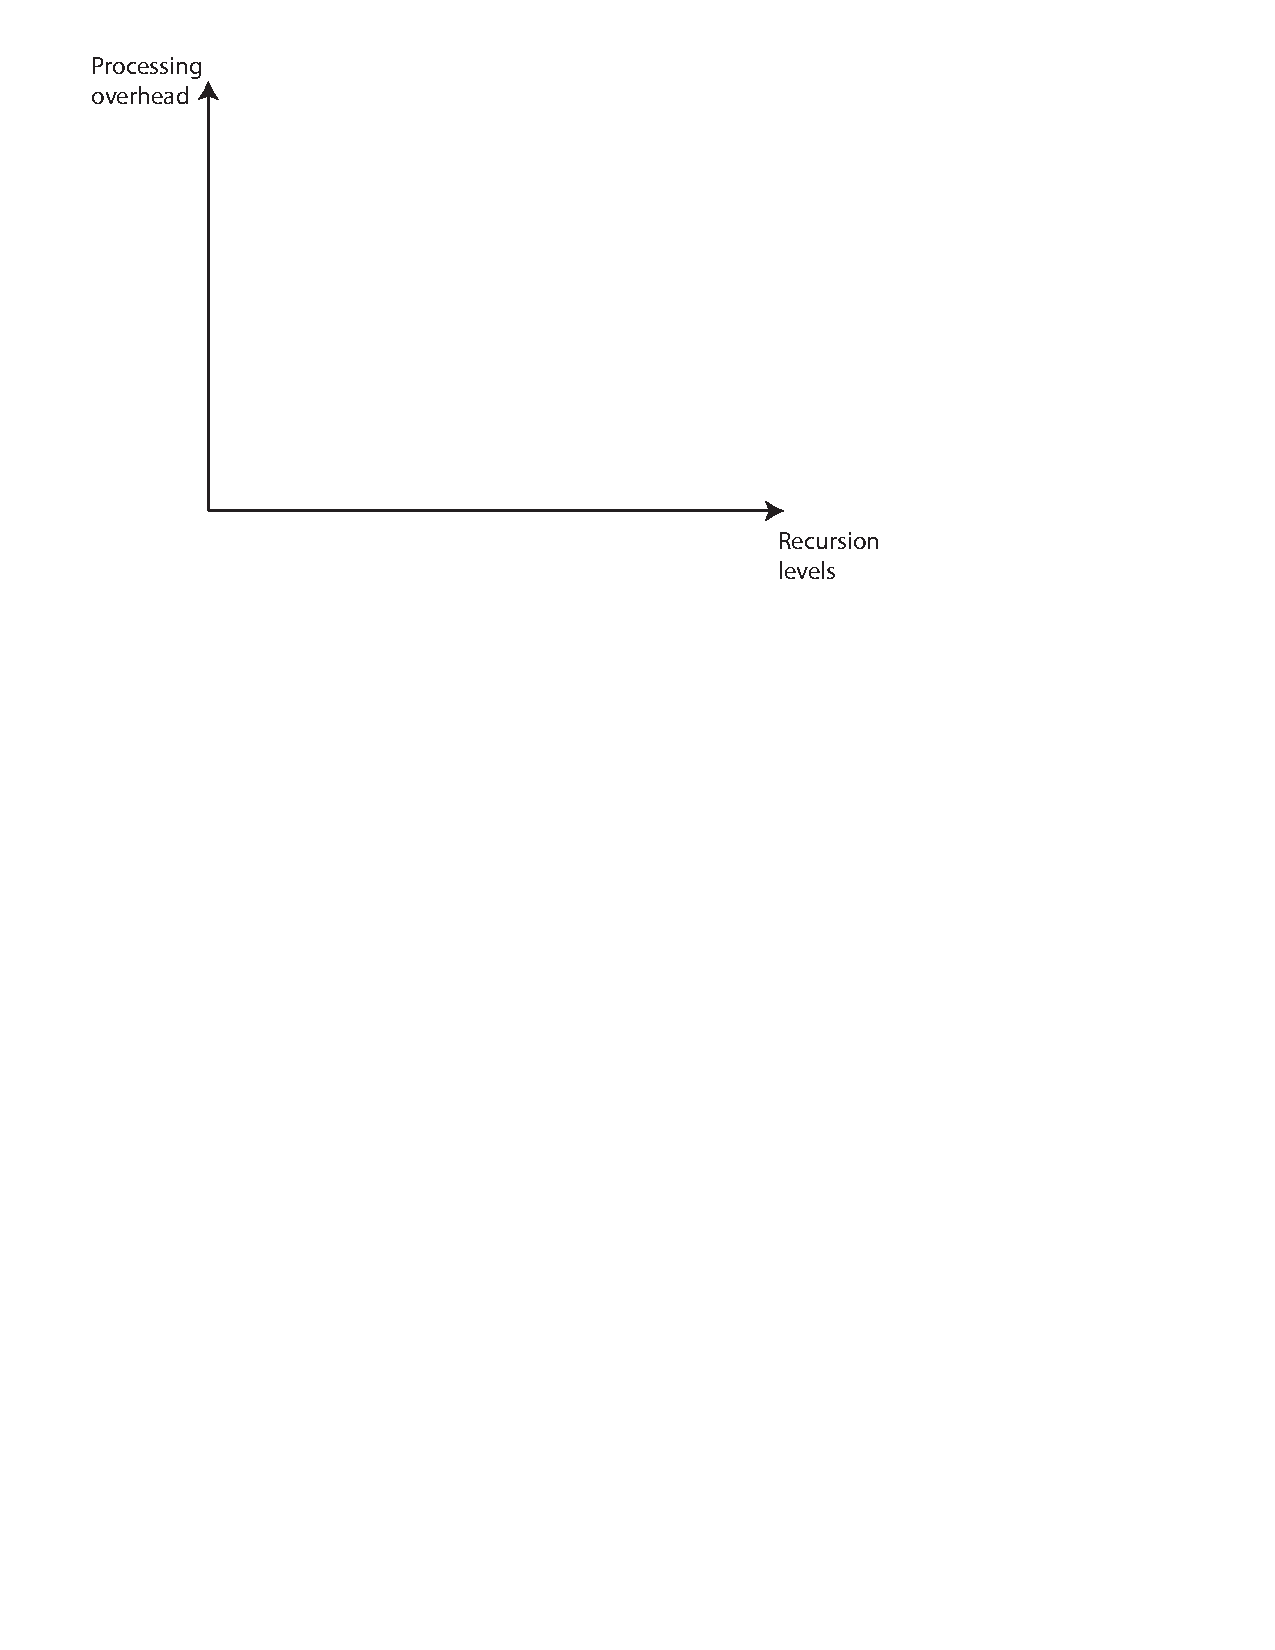
\includegraphics[scale=0.6]{figures/axes-rlevels.pdf}
\caption{Query processing overhead under varying degrees of recursive
compilation aggressiveness, for a \textit{k}-nested query.}
\label{fig:overhead-recursion-levels-nesting}
\end{figure}

\begin{figure}
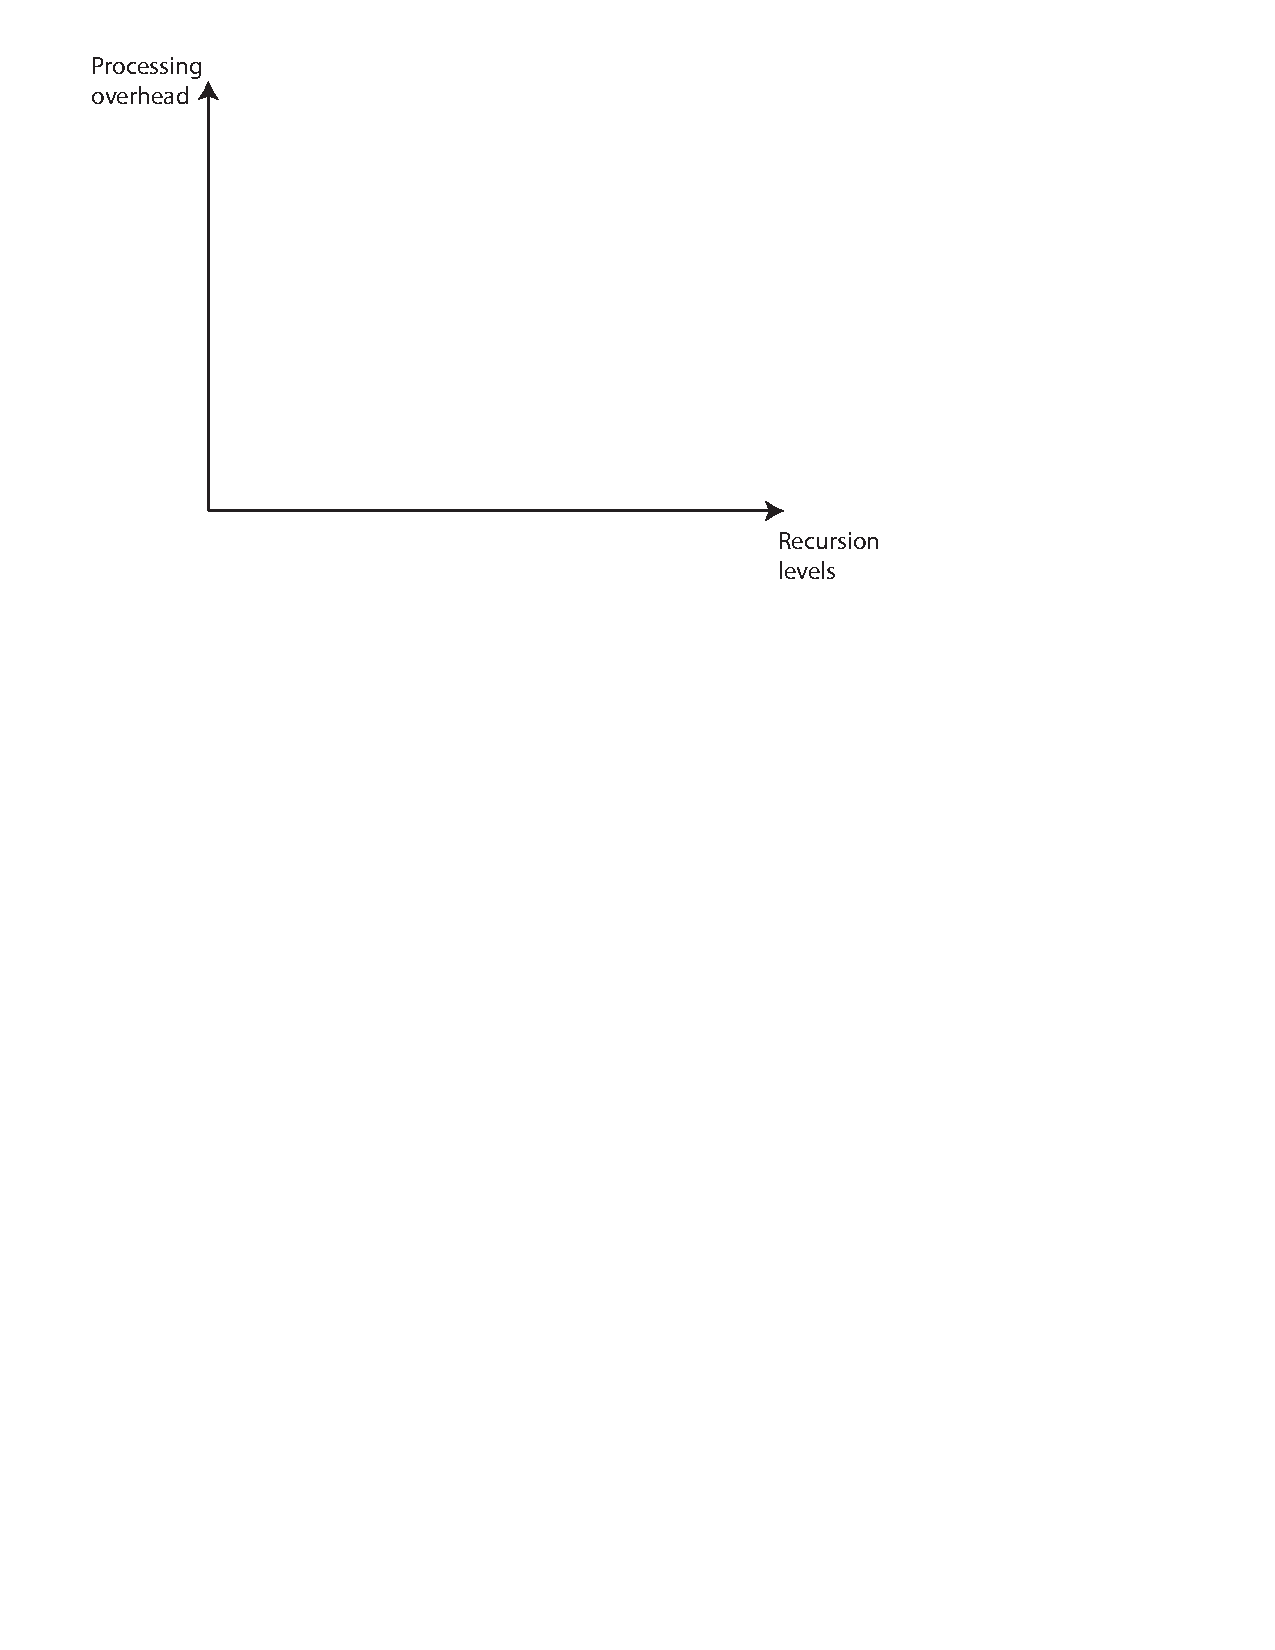
\includegraphics[scale=0.6]{figures/axes-rlevels.pdf}
\caption{Query processing overhead under varying degrees of recursive
compilation aggressiveness, for a \textit{k}-way join.}
\label{fig:overhead-recursion-levels-join}
\end{figure}

\begin{figure}
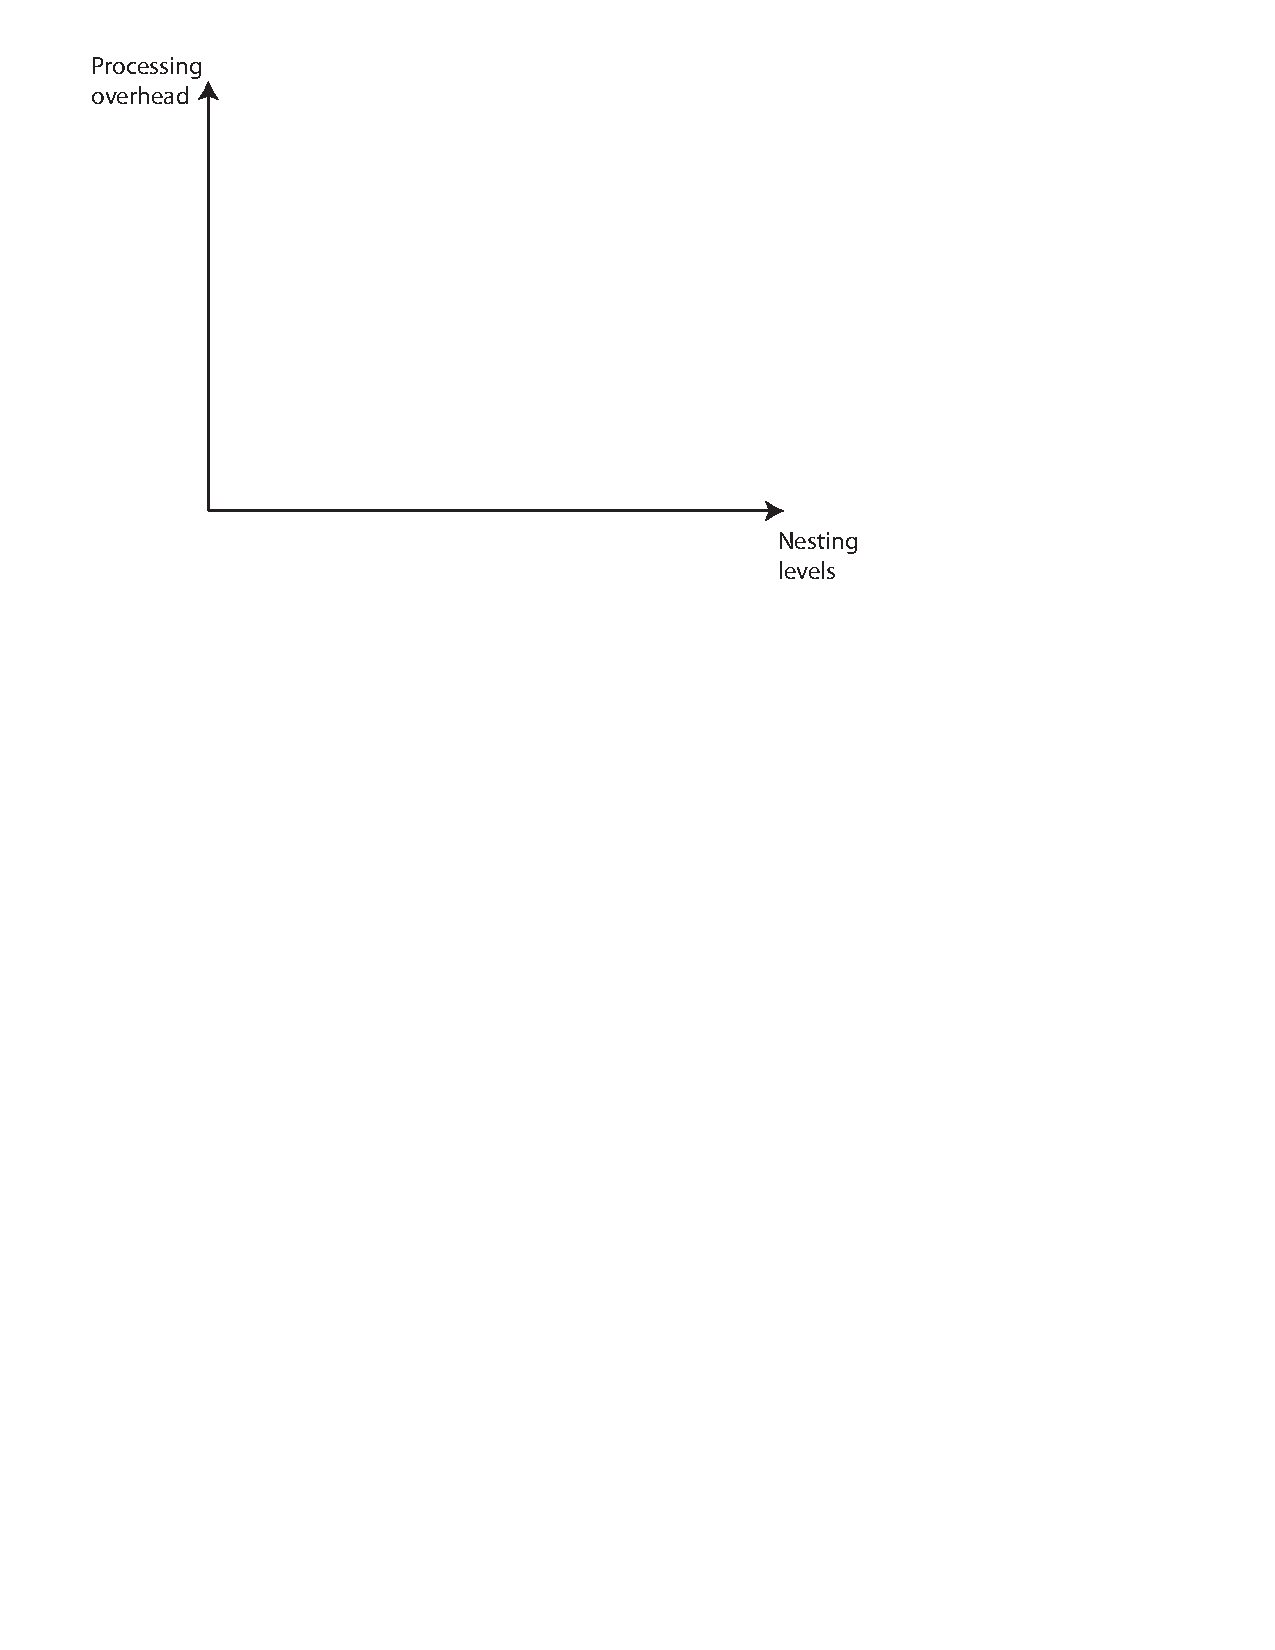
\includegraphics[scale=0.6]{figures/axes-nlevels.pdf}
\caption{Query processing overhead under varying nesting workloads, for
recursive compilation and incremental view maintenance.}
\label{fig:overhead-workload-nesting}
\end{figure}

\begin{figure}
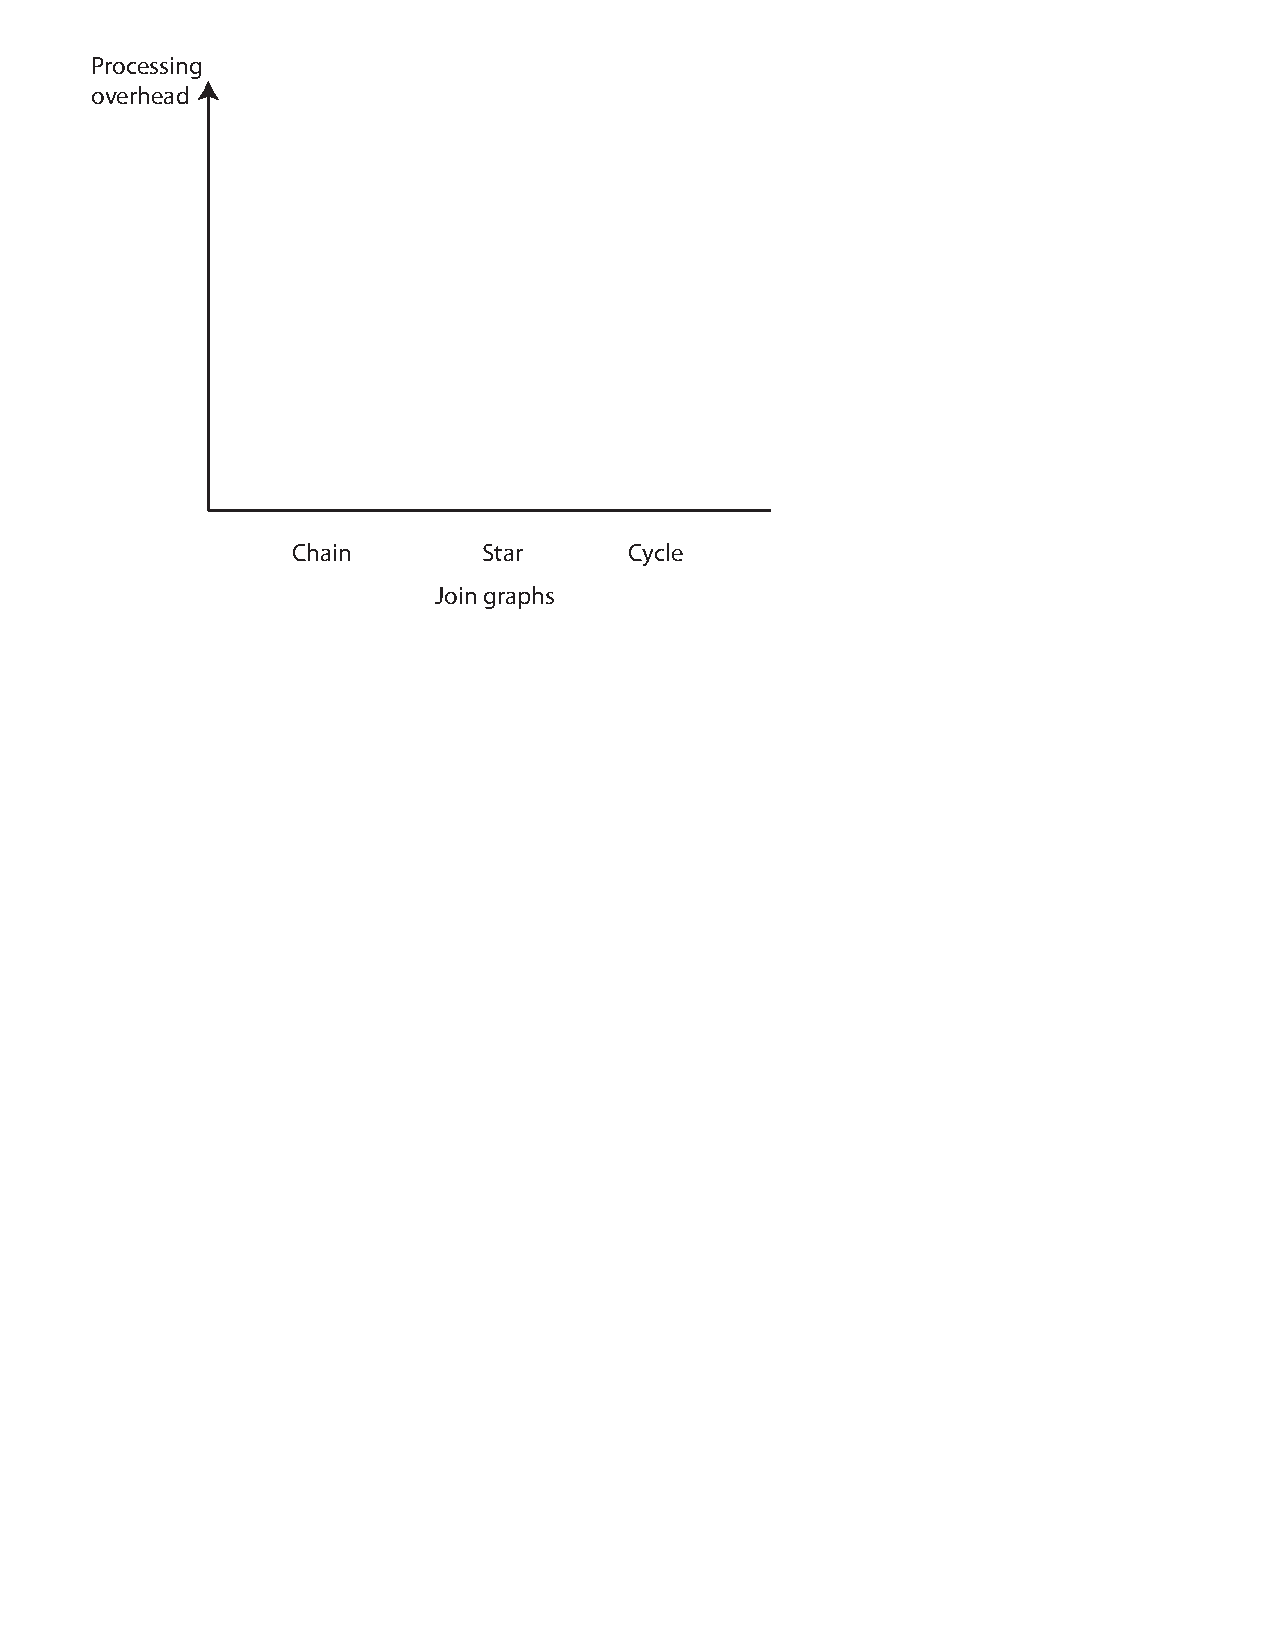
\includegraphics[scale=0.6]{figures/axes-jgraph.pdf}
\caption{Query processing overhead under varying join graph workloads for
recursive compilation and incremental view maintenance.}
\label{fig:overhead-workload-join}
\end{figure}

\subsubsection{Algorithmic Trading and Data Warehousing applications}
\begin{itemize}
\item Compare naive query processing and incremental view maintenance to full
DBToaster recursive compilation for real-world scenarios.
\end{itemize}

\begin{figure}
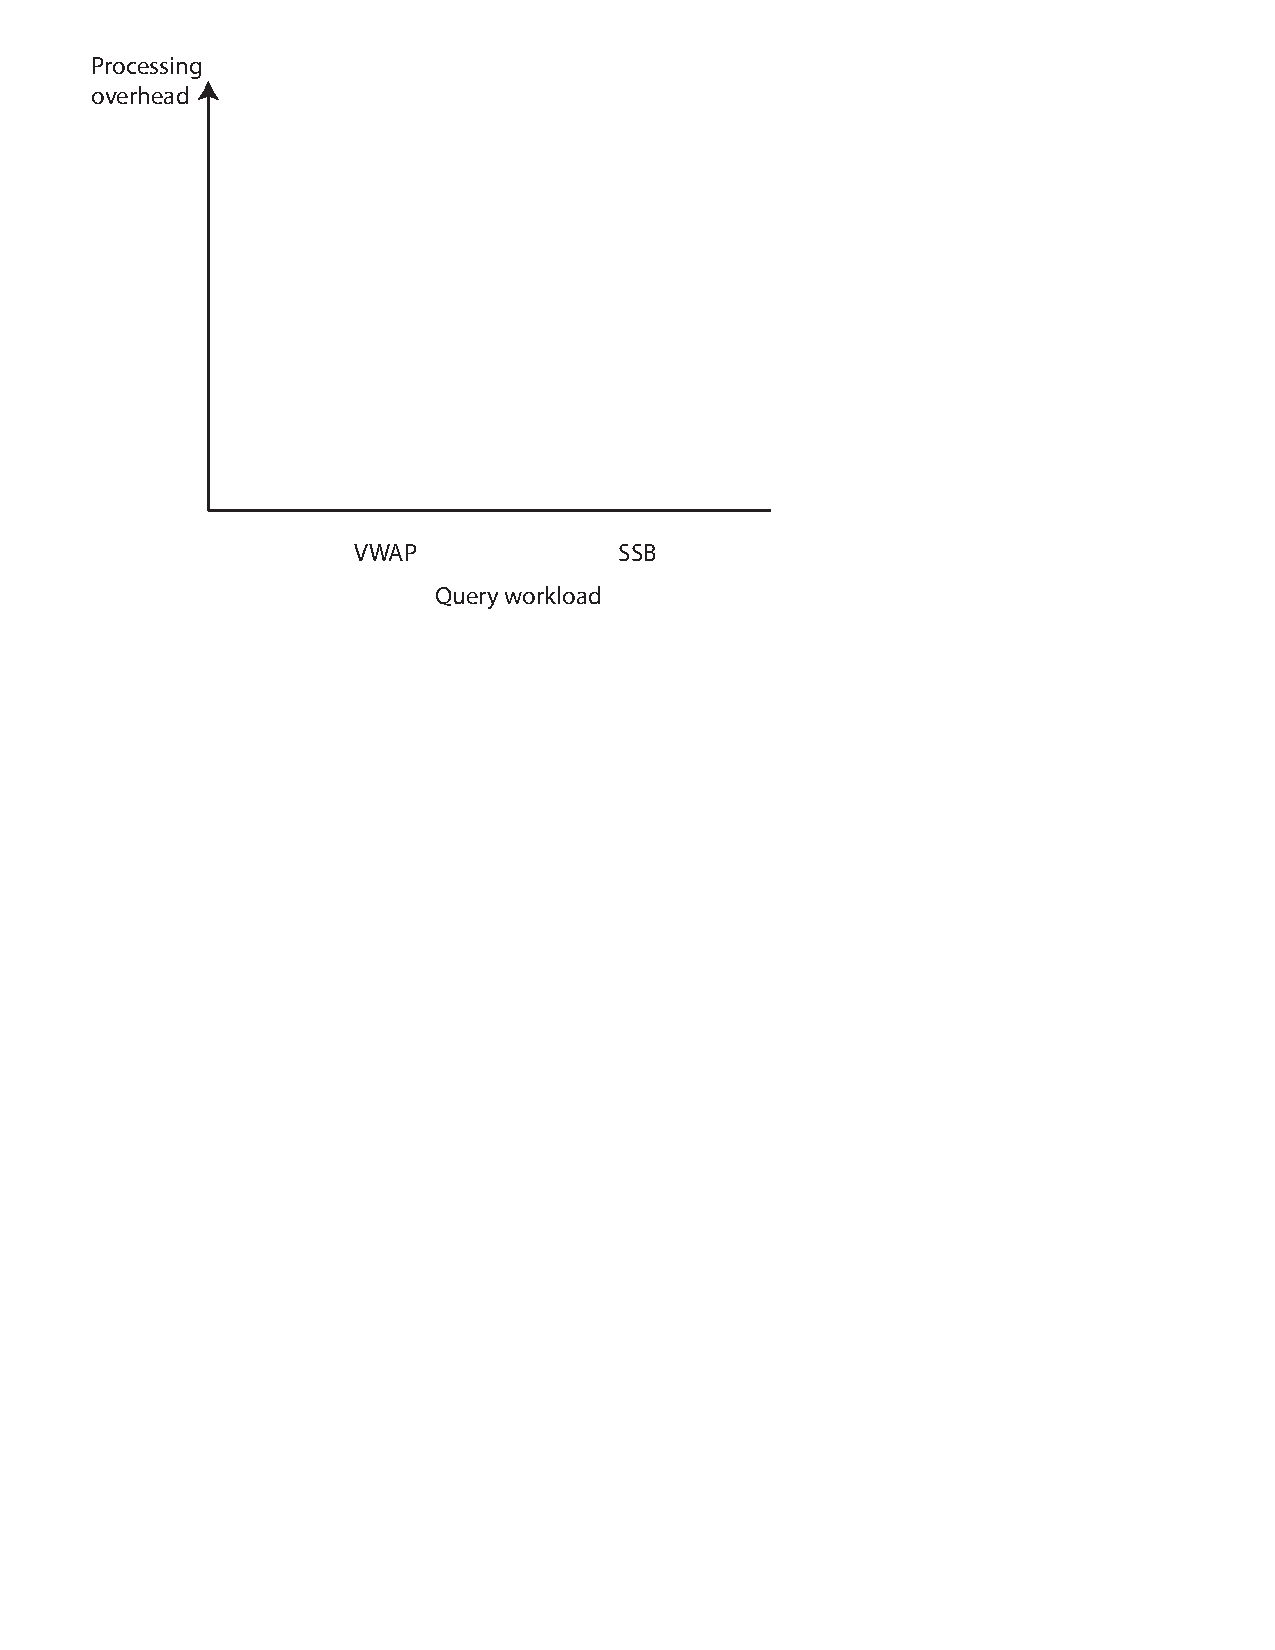
\includegraphics[scale=0.6]{figures/axes-query.pdf}
\caption{Query processing overheads for the VWAP and SSB queries, for naive
  query processing, incremental view maintenance and DBToaster.}
\label{fig:overhead-vwap-ssb}
\end{figure}

\subsection{Memory Utilization}
\begin{itemize}
\item Measure total process memory usage over time, taking samples every $k$
  tuples (find a suitable value of $k$, perhaps 1000?).
\item Use the following formula to estimate a std::map$<>$ memory usage:
\begin{align*}
(sizeof(key) & + sizeof(value) + \\
& sizeof(rb\_tree\_node))*N\\
+ sizeof(rb\_tree)
\end{align*}

\item If time permits, use a custom allocator with an identifier for each map
assigned to use the allocator to track memory usage per map.

\item We have the following formulae for the number of maps created for k-way
joins with specific types of join graphs. These are derived by considering the
combinations of subgraphs of size $i$ (which constitute relations we can
aggregate), with $i = [1 \ldots k-1]$
    \begin{itemize}
    \item Chain: $\sum_{i=1}^{k}{i} = \frac{k(k+1)}{2}$
    \item Star: $(\sum_{i=1}^{k-1}{\binom{k-1}{i}}) + k $
    \item Cycle: $k*\sum_{i=1}^{k-1}{i} = \frac{k^2(k-1)}{2}$
    \end{itemize}

\item Predicted memory utilization:
    \begin{itemize}
    \item VWAP: mem(DBToaster) $>$ mem(VM) $>$ mem(naive) -- due to increased
    map usage, while still needing to maintain full domain. This changes if the base
    relation contains many duplicates, i.e. $|dom(P)| << |bids|$.
    \end{itemize}
\end{itemize}

\begin{figure}
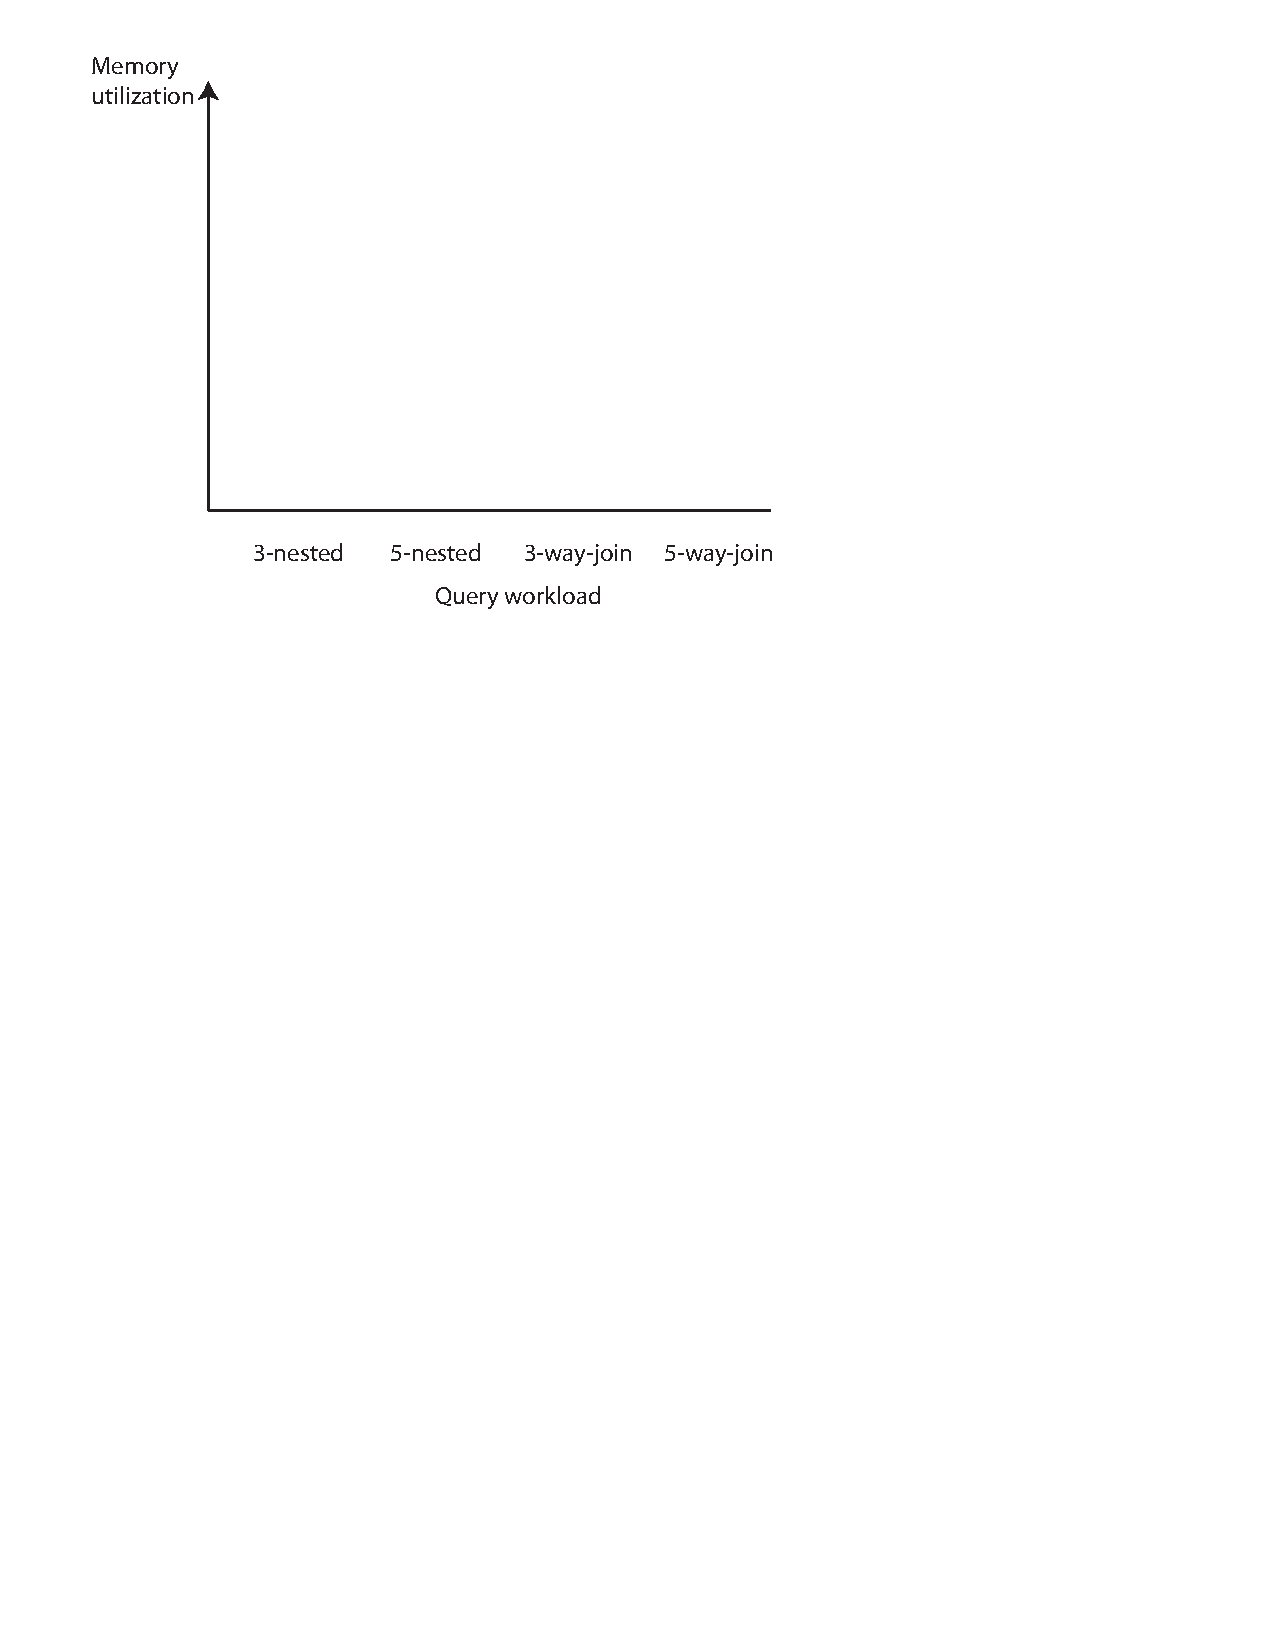
\includegraphics[scale=0.6]{figures/axes-memnjquery.pdf}
\caption{Memory utilization of the naive, incremental view maintenance, and
  DBToaster query processing techniques on nested and multiway join queries.}
\label{fig:memutil-njquery}
\end{figure}

\begin{figure}
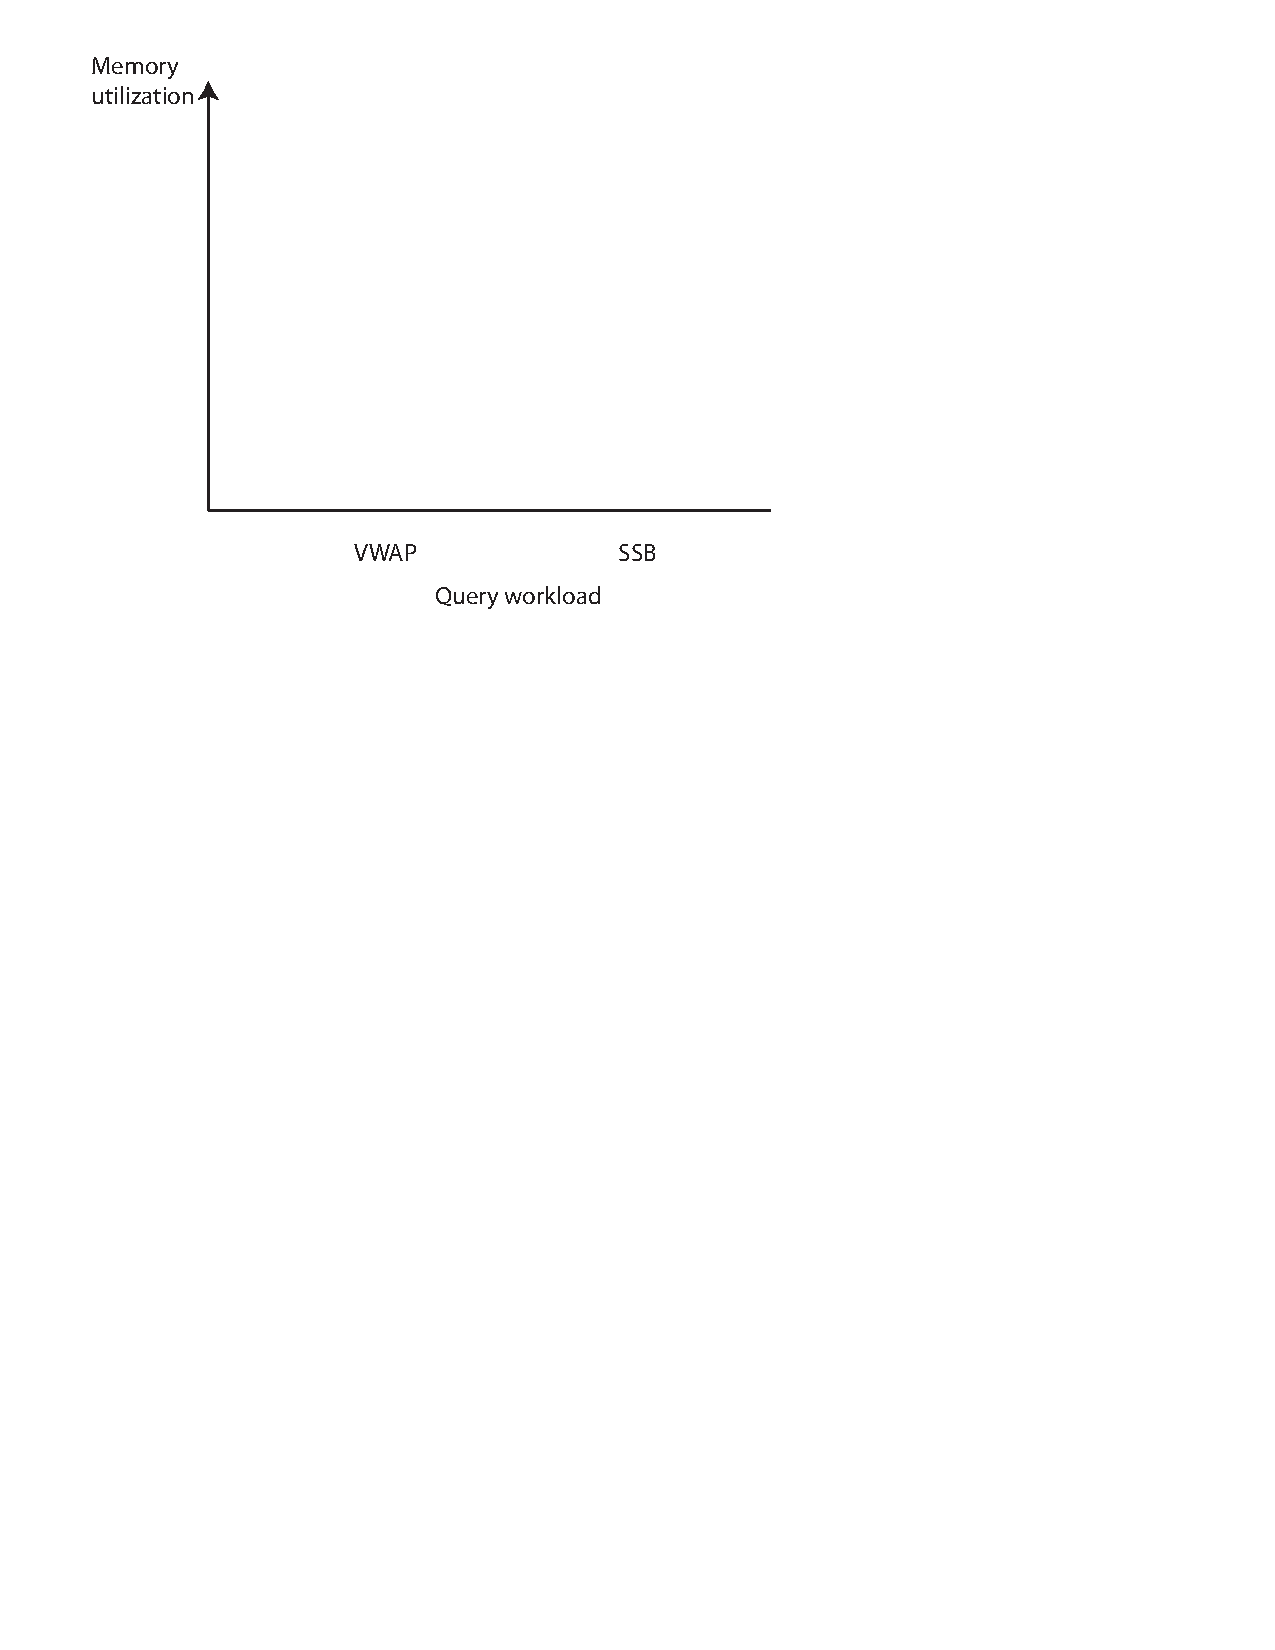
\includegraphics[scale=0.6]{figures/axes-memvsquery.pdf}
\caption{Memory utilization of the naive, incremental view maintenance, and
DBToaster query processing techniques for the VWAP and SSB queries.}
\label{fig:memutil-vsquery}
\end{figure}

\subsection{DBMS Bakeoff}
\begin{itemize}
\item Compare DBToaster to Postgres, HSQLDB, Oracle (DBMS 'X'), Borealis,
  Streambase (DBMS 'Y').
\item Compare using four different techniques: repetitive processing, trigger
  processing, builtin view maintenance, and stream processing.
\item What about a column store, e.g. Vertica/MonetDB? This would only be
  possible under a repetitive QP technique (or does Vertica implement triggers?)
\end{itemize}

\subsubsection{Repetitive Processing}
\begin{itemize}
\item Check whether we can simply pass through queries to Postgres, DBMS 'X' and
  HSQLDB, or whether it's better to generate from map algebra due to specific
  SQL syntax for each DBMS.
\item Run experiment for repeating at various fractions of the dataset size,
  i.e. 10\%,20\%,...,100\%, where 100\% means running the query for every tuple.
\item Note other DBMS can exploit caching here significantly, while DBToaster
  currently does not perform caching, and is L1/L2 cache-agnostic.
\end{itemize}

\begin{figure}
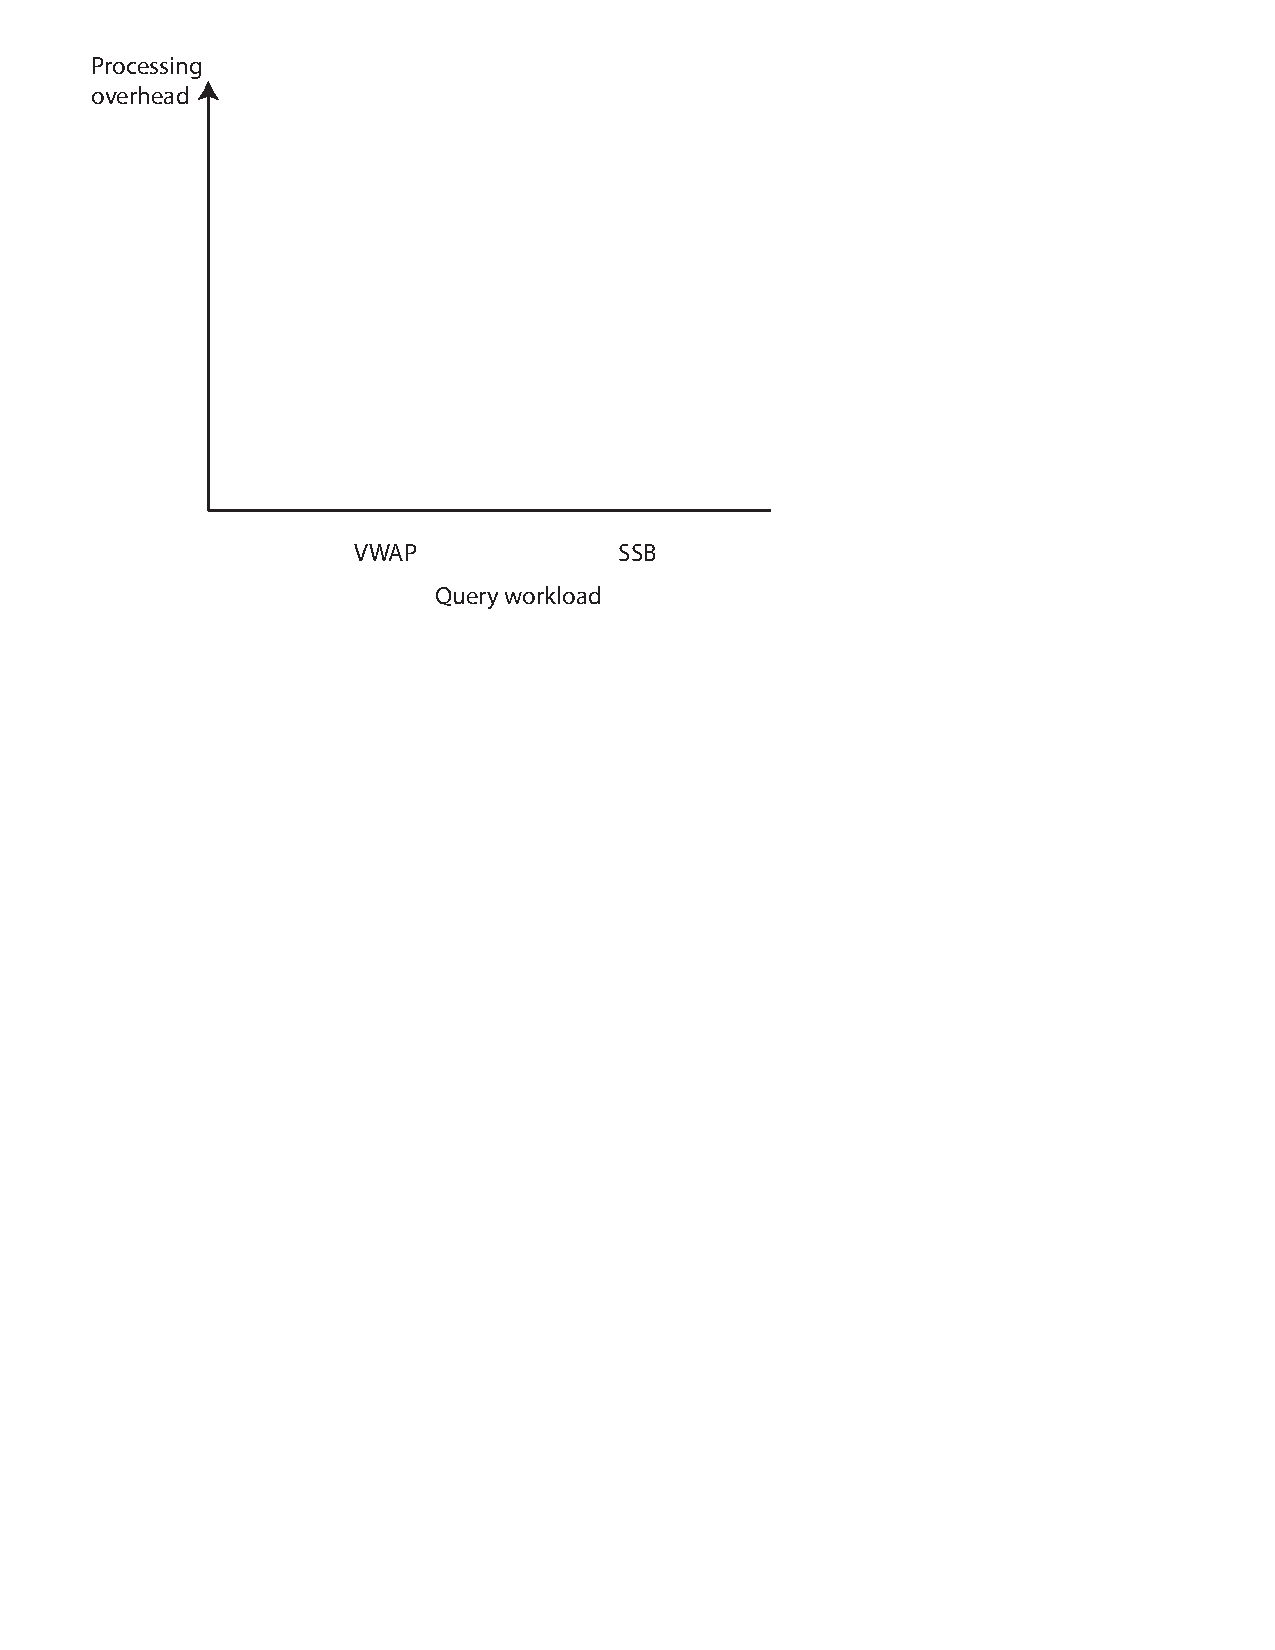
\includegraphics[scale=0.6]{figures/axes-repetitive.pdf}
\caption{Comparison of repetitive ad-hoc query processing of the VWAP and SSB
queries, in Postgres, DBMS 'X' and HSQLDB, to DBToaster's compiled query
processing.}
\label{fig:overhead-repetition}
\end{figure}

\subsubsection{Trigger-based processing}
\begin{itemize}
\item Generate trigger code from map algebra: use temporary tables as maps, and
  generate trigger code corresponding to each handler function.
\item HSQLDB only has Java-based triggers. Let's skip generating such Java-based
  triggers for now.
\item Postgres only allows row-based triggers to inspect tuple contents, DBMS
  'X' may allow access to the old and new tuple sets, allowing set-based
  triggering (like SQL Server).
\end{itemize}

\begin{figure}
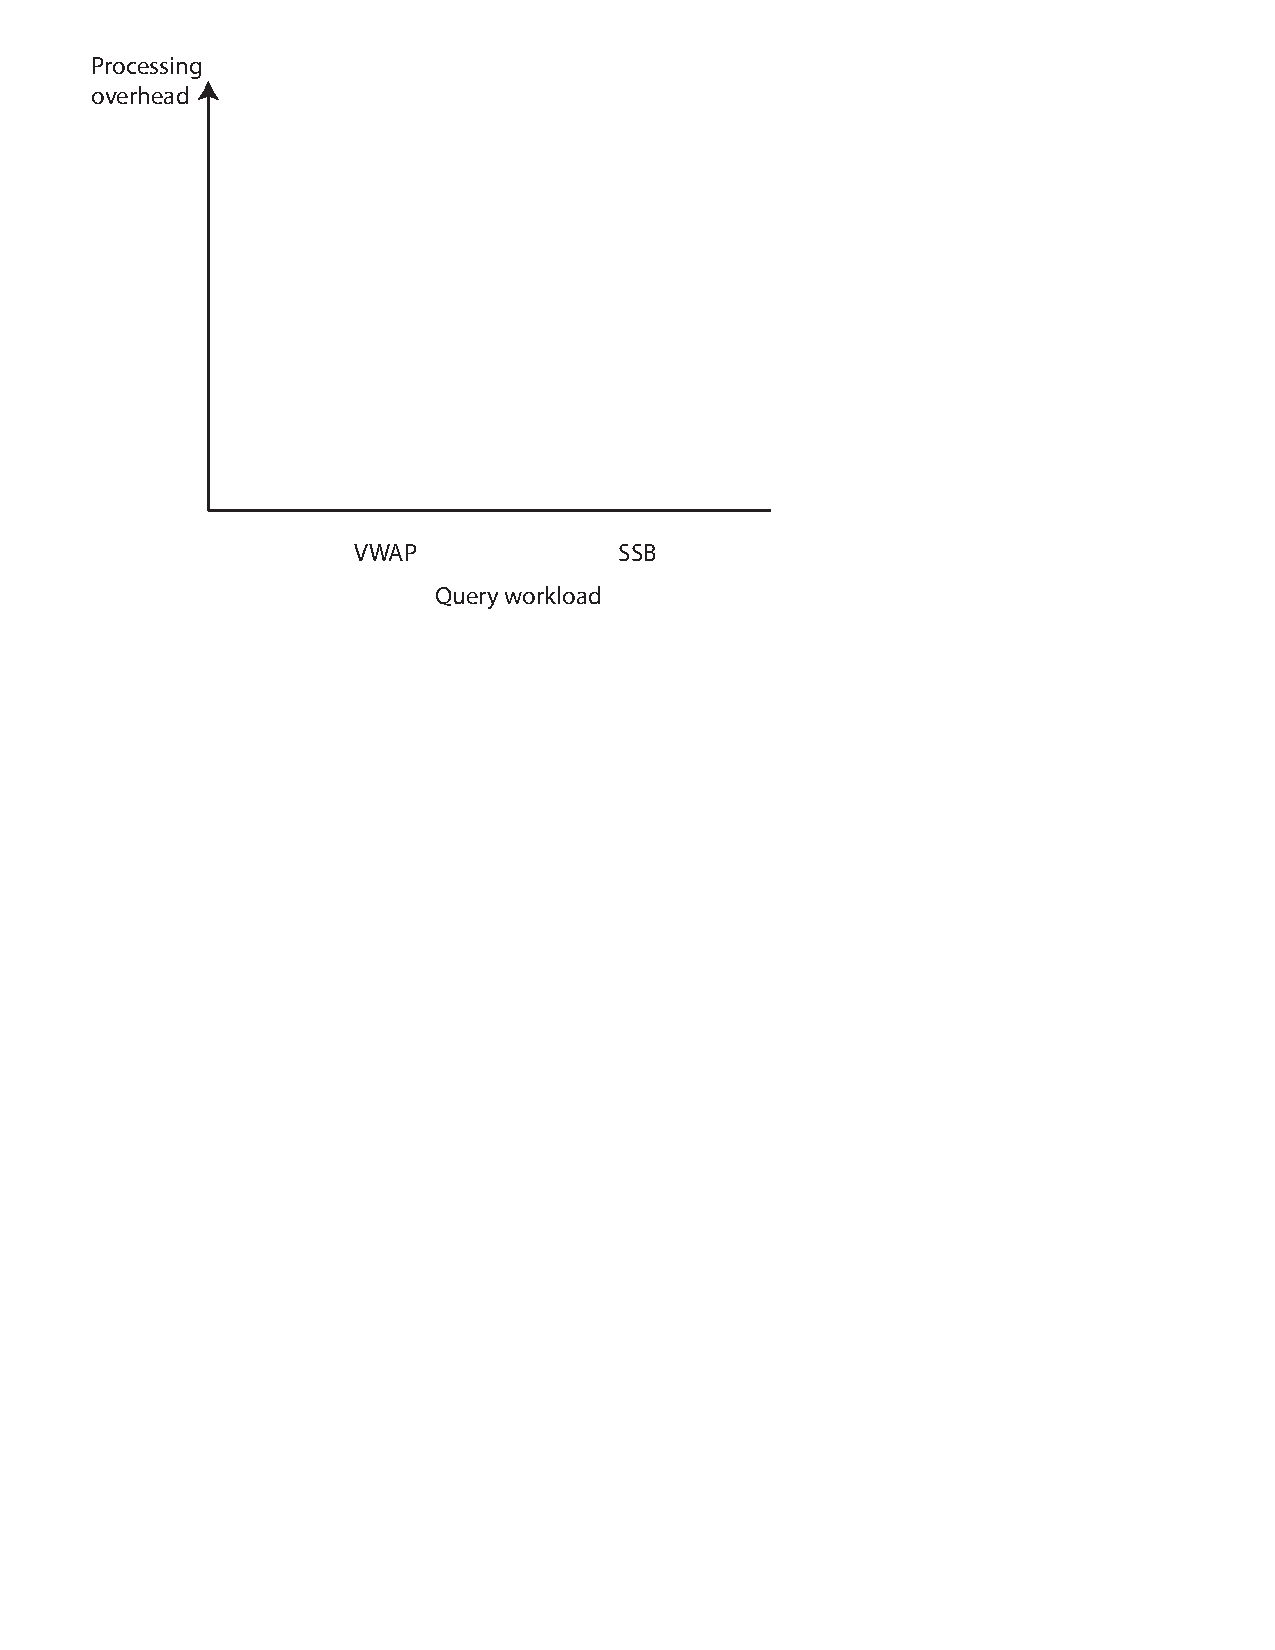
\includegraphics[scale=0.6]{figures/axes-triggers.pdf}
\caption{Comparison of trigger-based processing of the VWAP and SSB queries in
Postgres, DBMS 'X' and HSQLDB to DBToaster's compiled query processing}
\label{fig:overhead-trigger}
\end{figure}

\subsubsection{Materialized view maintenance}
\begin{itemize}
\item Pick a feasible query for view maintenance (perhaps TPCH/SSB queries...) since
  VWAP cannot be done via incremental view maintenance in DBMS 'X'.
\item Check if we can simply pass through user-specified query to DBMS 'X's create
  view DDL statement.
\end{itemize}

\begin{figure}
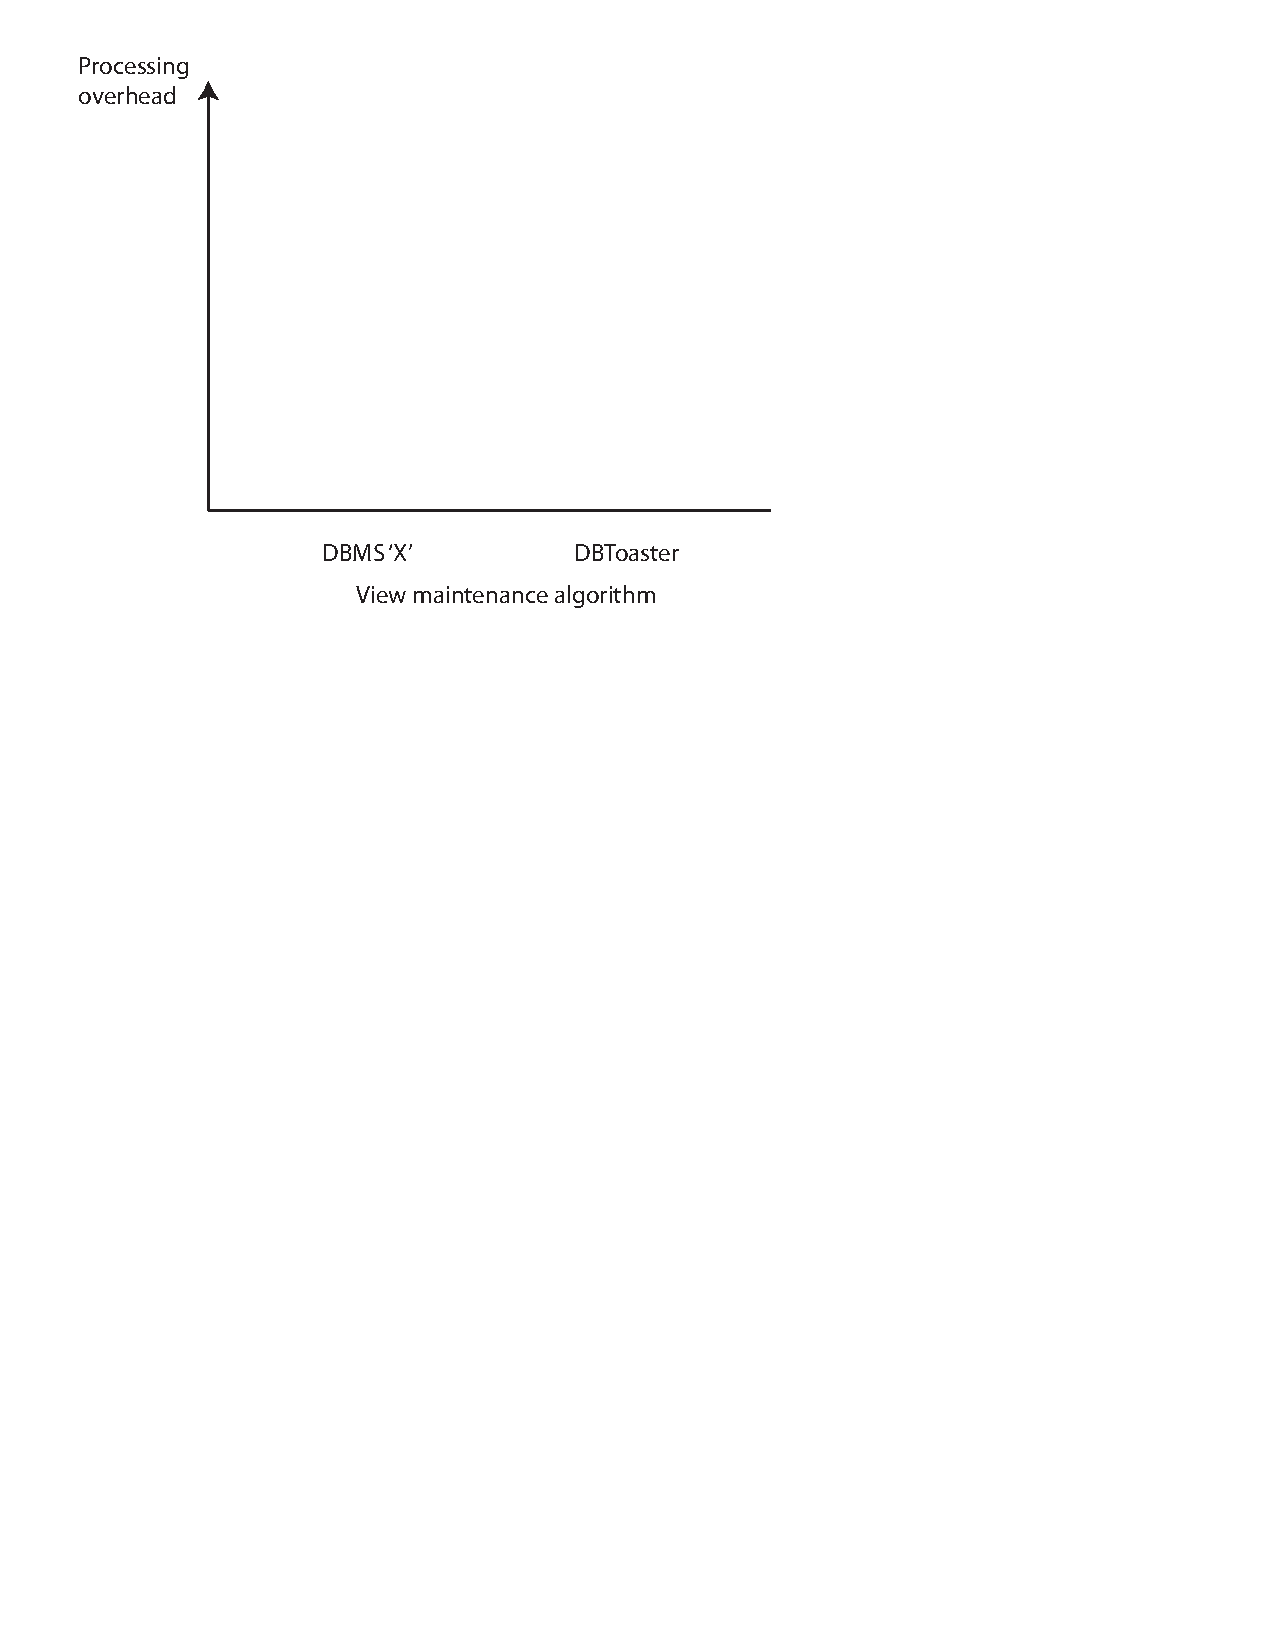
\includegraphics[scale=0.6]{figures/axes-views.pdf}
\caption{Comparison of view maintenance in DBMS 'X' to DBToaster's compiled query processing}
\label{fig:overhead-trigger}
\end{figure}

\subsubsection{Stream processing}
\begin{itemize}
\item Pick a feasible query for stream processing (i.e., pure stream processing
  query, perhaps Linear Road avg lav), that does not require the use of
  in-memory tables.
\item Compare both VWAP query and pure-stream query (i.e. with windowing
  expressed as a range predicate in DBToaster).
\item Generate Borealis XML representation and Streambase app XML representation
  directly from initial map algebra.
\end{itemize}

\begin{figure}
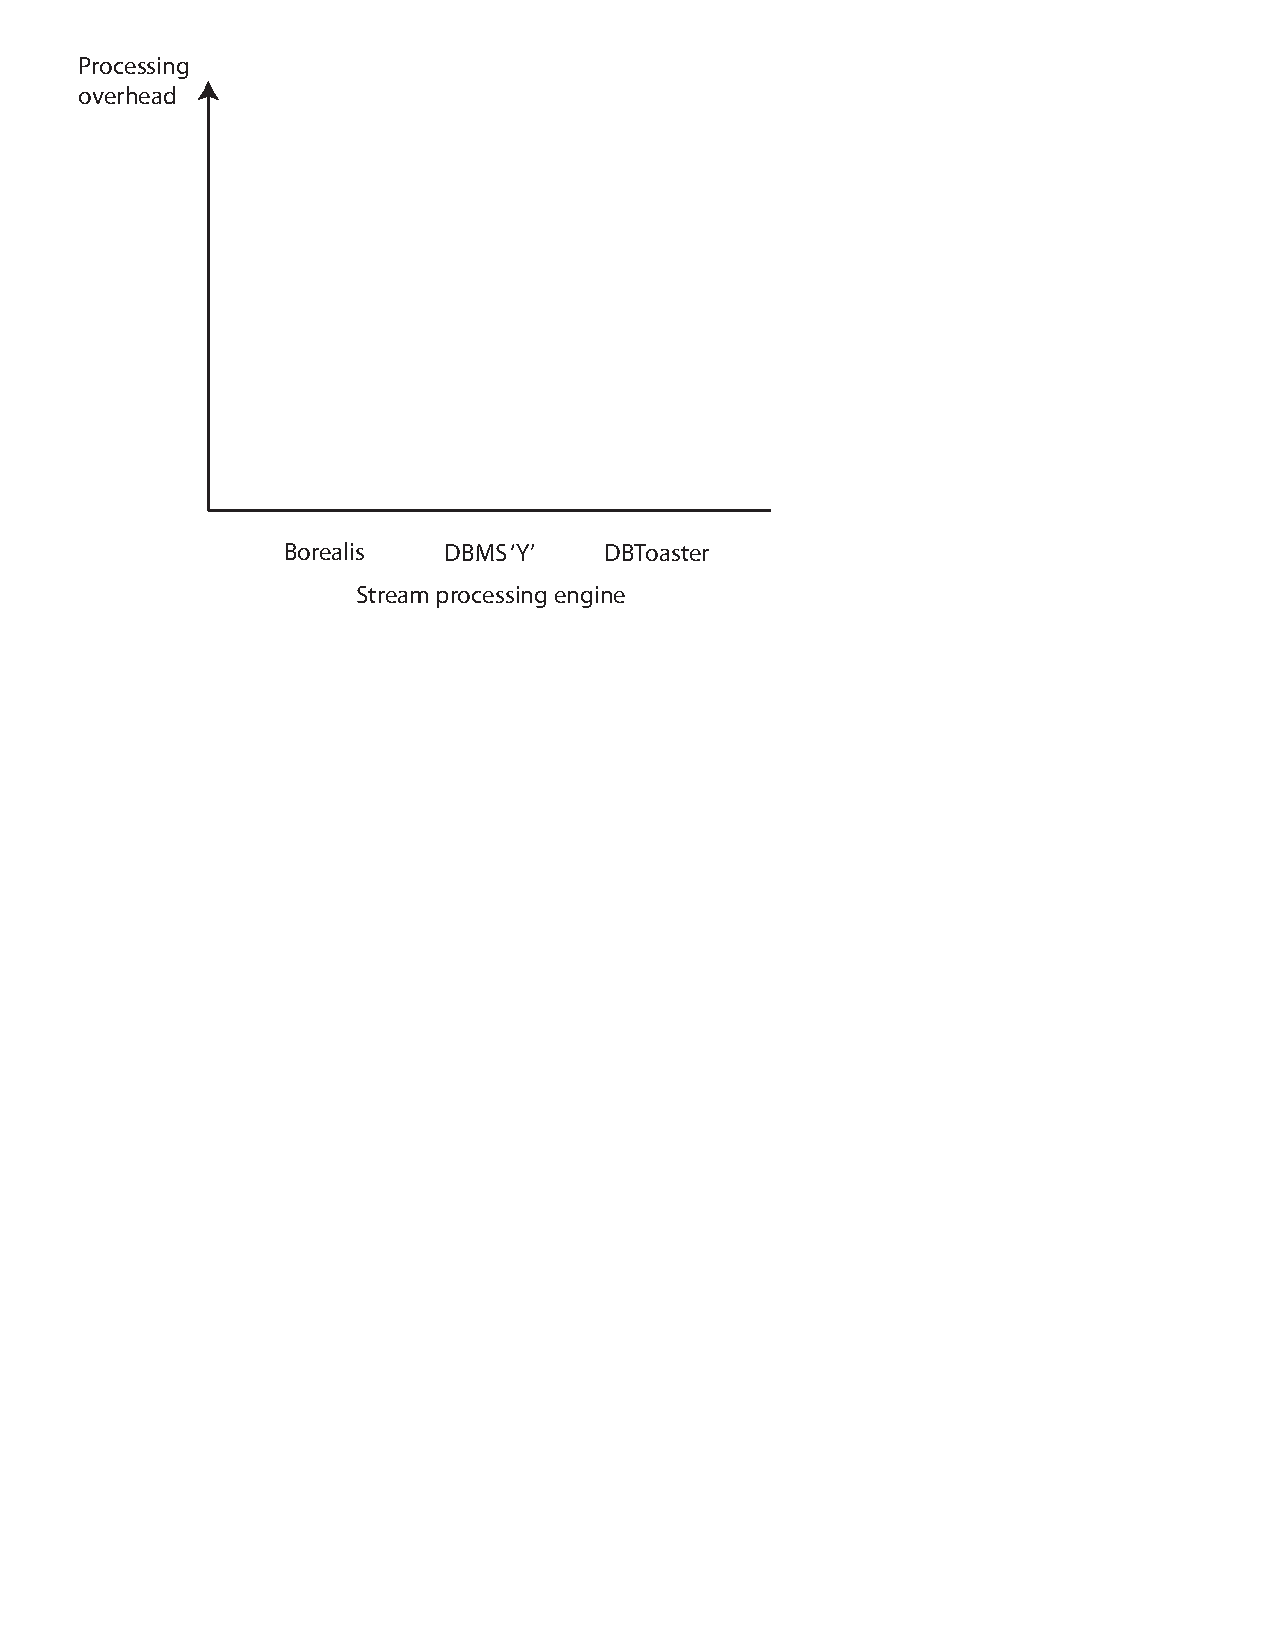
\includegraphics[scale=0.6]{figures/axes-streams.pdf}
\caption{Comparison of stream processing implementations of the XXX query, for
  Borealis and DBMS 'Y' to DBToaster's compiled query processing.}
\label{fig:overhead-stream}
\end{figure}

\subsection{DBToaster Cost Model}

\section{Related Work}

\section{Conclusions}

\end{document}